\documentclass[a4paper,11pt]{article}

% ---------- Packages ----------
\usepackage[margin=2.5cm]{geometry}
\usepackage{amsmath, amssymb, amsthm, mathtools}
\usepackage{algorithm}
\usepackage{algpseudocode}
\usepackage{enumitem}
\usepackage{graphicx}
\usepackage{booktabs}
\usepackage{hyperref}
\usepackage{xcolor}

\usepackage{tikz}
\usetikzlibrary{automata,positioning,arrows.meta}

% ---------- Theorem Environments ----------
\newtheorem{theorem}{Theorem}
\newtheorem{lemma}{Lemma}
\newtheorem{definition}{Definition}
\newtheorem{proposition}{Proposition}
\newtheorem{corollary}{Corollary}

% ---------- Custom Commands ----------
\newcommand{\R}{\mathbb{R}}
\newcommand{\N}{\mathbb{N}}
\newcommand{\Z}{\mathbb{Z}}
\newcommand{\Alphabet}{\Sigma}
\newcommand{\eps}{\varepsilon}
\newcommand{\set}[1]{\left\{ #1 \right\}}
\newcommand{\abs}[1]{\left| #1 \right|}
\newcommand{\ceil}[1]{\left\lceil #1 \right\rceil}
\newcommand{\floor}[1]{\left\lfloor #1 \right\rfloor}

% ---------- Section Style ----------
\renewcommand{\thesubsection}{(\alph{subsection})}
\renewcommand{\thesection}{}\renewcommand{\thesubsection}{(\alph{subsection})}

% ---------- Algorithm Style ----------
\algrenewcommand\algorithmicrequire{\textbf{Input:}}
\algrenewcommand\algorithmicensure{\textbf{Output:}}

% ---------- Title Info ----------
\title{\textbf{CSE2315 — Assignment 2}}
\author{Vlad Paun \\ 6152937}
\date{\today}

% ---------- Document ----------
\begin{document}

	\maketitle
	%\thispagestyle{empty}
	%\newpage

	\section{Exercise 1}
	Consider the language $L = (a^*b)^*$. Construct an NFA $N$ for which $L(N) = L$. To this end, answer the following:
	\subsection{Construct an NFA $N_1$ for which $L(N_1) = \set{x}$.}
	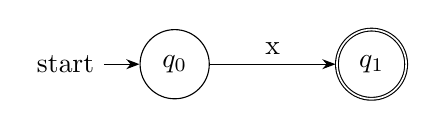
\begin{tikzpicture}[->, >=Stealth, auto, node distance=2.5cm]
		\node[initial,state] (q0) {$q_0$};
		\node[accepting,state] (q1) [right of=q0] {$q_1$};

		\path
		(q0) edge node {x} (q1);
	\end{tikzpicture}
	\subsection{Construct $N$ in a systematic way starting from $N_1$.}
	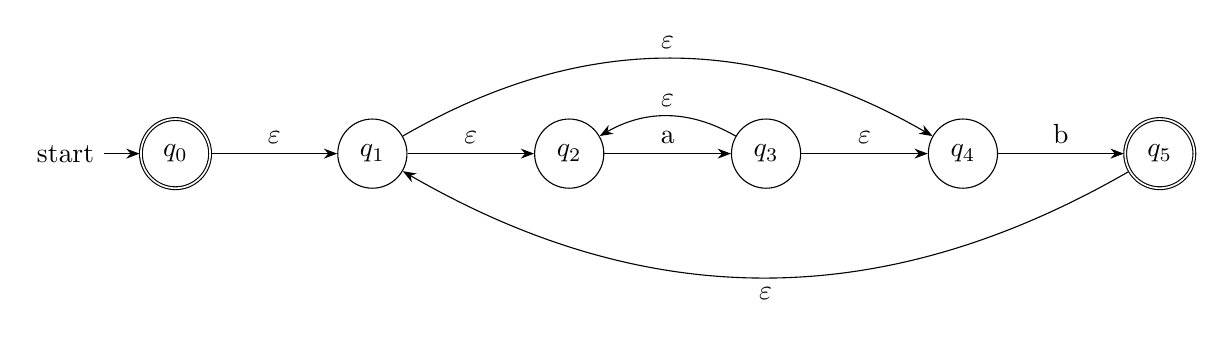
\begin{tikzpicture}[->, >=Stealth, auto, node distance=2.5cm]
		\node[initial, accepting, state] (q0) {$q_0$};

		\node[state] (q1) [right of=q0] {$q_1$};
		\node[state] (q2) [right of=q1] {$q_2$};
		\node[state] (q3) [right of=q2] {$q_3$};

		\node[state] (q4) [right of=q3] {$q_4$};
		\node[accepting, state] (q5) [right of=q4] {$q_5$};

		\path (q2) edge node {a} (q3);
		\path (q1) edge node {$\varepsilon$} (q2);
		\path (q3) edge [bend right] node [above] {$\varepsilon$}(q2);

		\path (q4) edge node {b} (q5);

		\path (q3) edge node {$\varepsilon$}(q4);
		\path (q1) edge [bend left] node {$\varepsilon$}(q4);

		\path (q0) edge node {$\varepsilon$} (q1);
		\path (q5) edge [bend left] node {$\varepsilon$} (q1);
	\end{tikzpicture}


	\section{Exercise 2}
	Consider the NFA $N=\set{\set{q_0,q_1,q_2},\set{a,b,c},\delta,q_0,\set{q_1,q_2}}$ depicted below:\\
	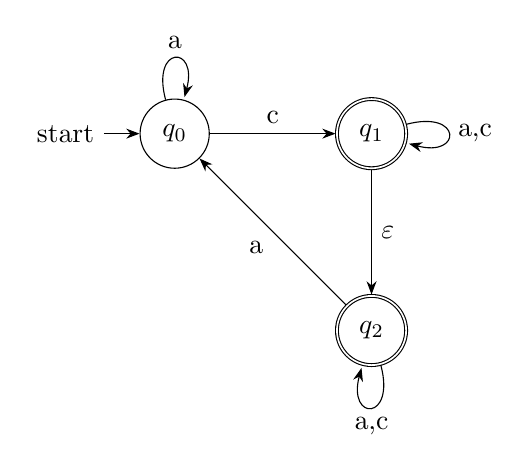
\begin{tikzpicture}[->, >=Stealth, auto, node distance=2.5cm]
		\node[initial, state] (q0) {$q_0$};
		\node[state,accepting] (q1) [right of=q0] {$q_1$};
		\node[state,accepting] (q2) [below of=q1] {$q_2$};

		\path (q0) edge [loop above] node {a} (q0);
		\path (q0) edge node {c} (q1);
		\path (q1) edge [loop right] node {a,c} (q1);
		\path (q1) edge node {$\varepsilon$} (q2);
		\path (q2) edge [loop below] node {a,c} (q2);
		\path (q2) edge node {a} (q0);
	\end{tikzpicture}\\
	Construct a DFA $D$ such that $L(D) = L(N)$:

	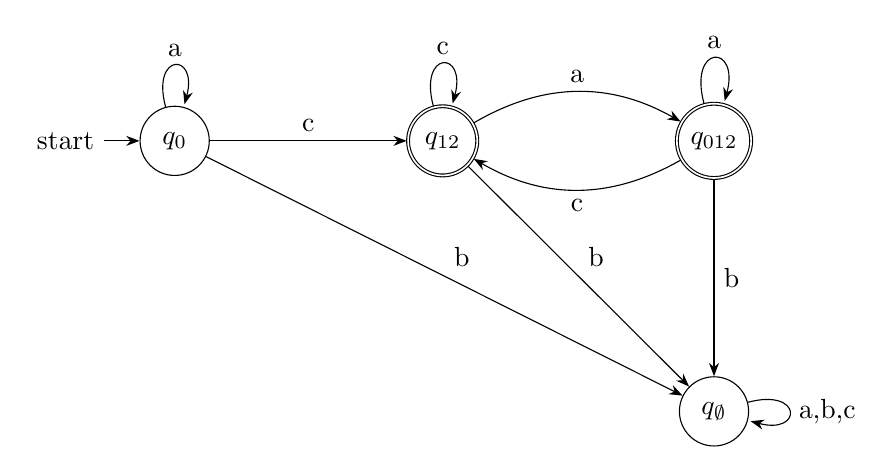
\begin{tikzpicture}[->, >=Stealth, auto, node distance=2.5cm]
		\node[initial,state] (q0) {$q_0$};
		\node[state,accepting, right=of q0] (q12) {$q_{12}$};

		\node[state,accepting, right=of q12] (q012) {$q_{012}$};
		\node[state, below=of q012] (qempty) {$q_{\emptyset}$};

		\path (q0) edge [loop above] node {a} (q0);
		\path (q0) edge node {b} (qempty);
		\path (q0) edge node {c} (q12);

		\path (q12) edge [bend left] node {a} (q012);
		\path (q12) edge node {b} (qempty);
		\path (q12) edge [loop above] node {c} (q12);

		\path (q012) edge [loop above] node {a} (q012);
		\path (q012) edge node {b} (qempty);
		\path (q012) edge [bend left]node {c} (q12);

		\path (qempty) edge [loop right] node {a,b,c} (qempty);
	\end{tikzpicture}


	\iffalse
	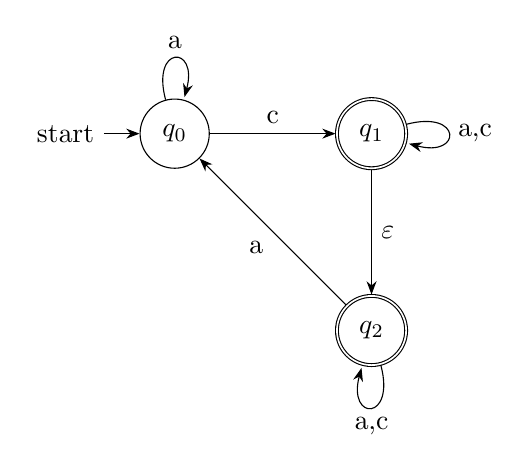
\begin{tikzpicture}[->, >=Stealth, auto, node distance=2.5cm]
		\node[initial, state] (q0) {$q_0$};
		\node[state,accepting] (q1) [right of=q0] {$q_1$};
		\node[state,accepting] (q2) [below of=q1] {$q_2$};

		\path (q0) edge [loop above] node {a} (q0);
		\path (q0) edge node {c} (q1);
		\path (q1) edge [loop right] node {a,c} (q1);
		\path (q1) edge node {$\varepsilon$} (q2);
		\path (q2) edge [loop below] node {a,c} (q2);
		\path (q2) edge node {a} (q0);
	\end{tikzpicture}\\
	Construct a DFA $D$ such that $L(D) = L(N)$:

	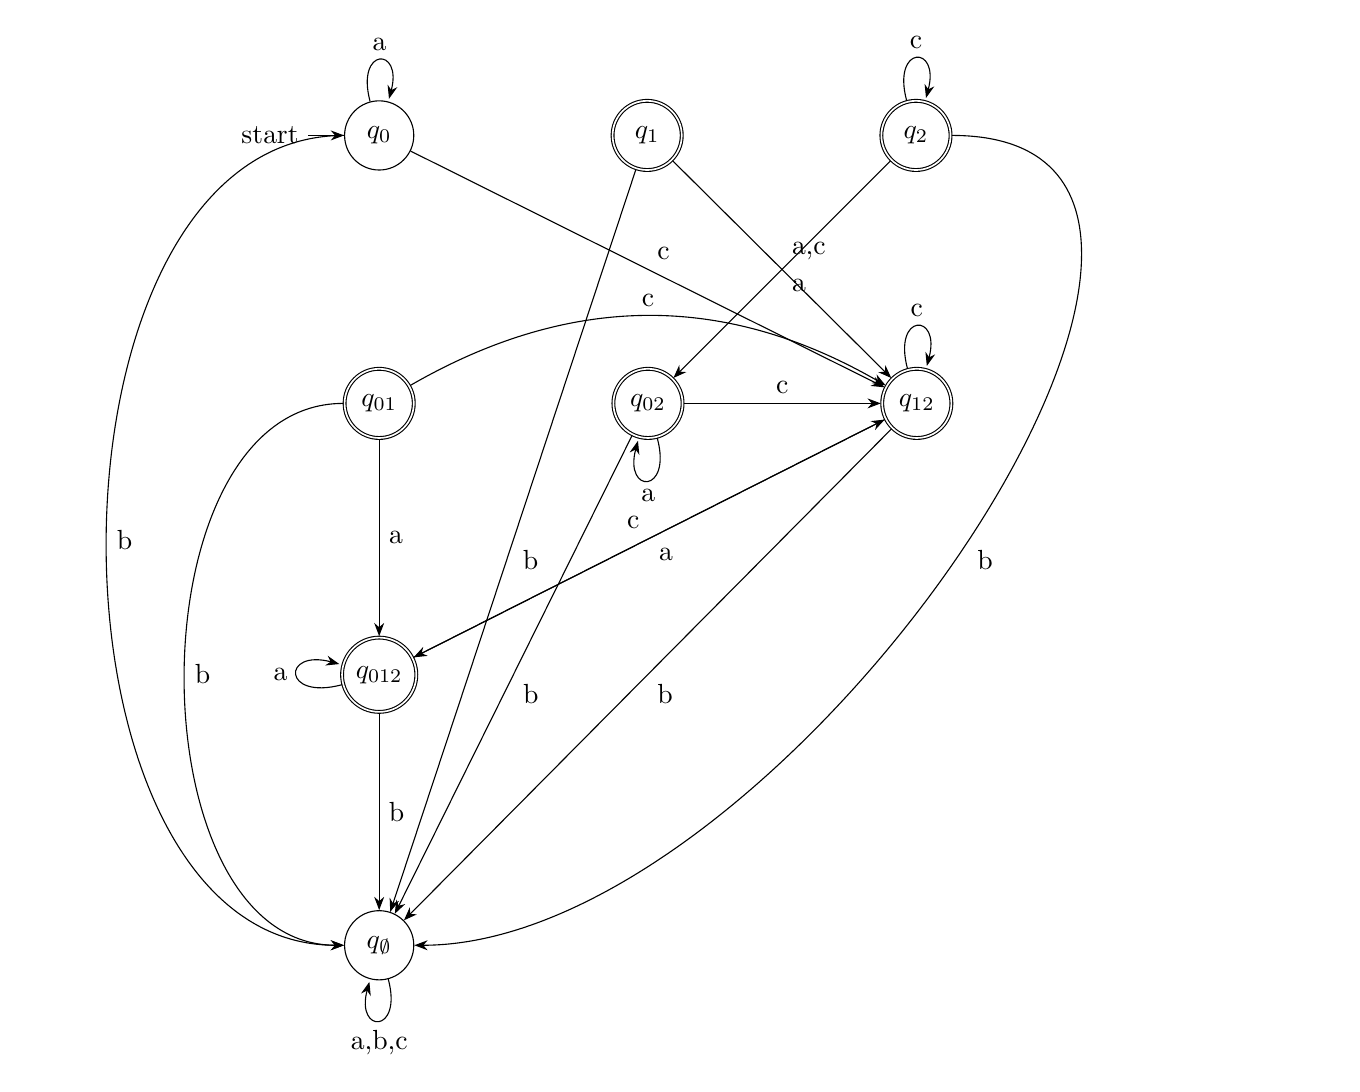
\begin{tikzpicture}[->, >=Stealth, auto, node distance=2.5cm]
		\node[initial,state] (q0) {$q_0$};
		\node[state,accepting, right=of q0] (q1) {$q_1$};
		\node[state,accepting, right=of q1] (q2) {$q_2$};

		\node[state,accepting, below=of q0] (q01) {$q_{01}$};
		\node[state,accepting, right=of q01] (q02) {$q_{02}$};
		\node[state,accepting, right=of q02] (q12) {$q_{12}$};

		\node[state,accepting, below=of q01] (q012) {$q_{012}$};
		\node[state, below=of q012] (qempty) {$q_{\emptyset}$};

		\path (q0) edge [loop above] node {a} (q0);
		\path (q0) edge [out=180,in=180] node {b} (qempty);
		\path (q0) edge node {c} (q12);

		\path (q1) edge node {a,c} (q12);
		\path (q1) edge node {b} (qempty);

		\path (q2) edge node {a} (q02);
		\path (q2) edge [out=0,in=0] node {b} (qempty);
		\path (q2) edge [loop above] node {c} (q2);

		\path (q01) edge node {a} (q012);
		\path (q01) edge [out=180,in=180] node {b} (qempty);
		\path (q01) edge [bend left]node {c} (q12);

		\path (q02) edge [loop below] node {a} (q02);
		\path (q02) edge node {b} (qempty);
		\path (q02) edge node {c} (q12);

		\path (q12) edge node {a} (q012);
		\path (q12) edge node {b} (qempty);
		\path (q12) edge [loop above] node {c} (q12);

		\path (q012) edge [loop left] node {a} (q012);
		\path (q012) edge node {b} (qempty);
		\path (q012) edge node {c} (q12);

		\path (qempty) edge [loop below] node {a,b,c} (qempty);
	\end{tikzpicture}
	\fi


	\section{Exercise 3}
	Consider the following two DFAs $D_1$,$D_2$:\\
	\begin{center}
		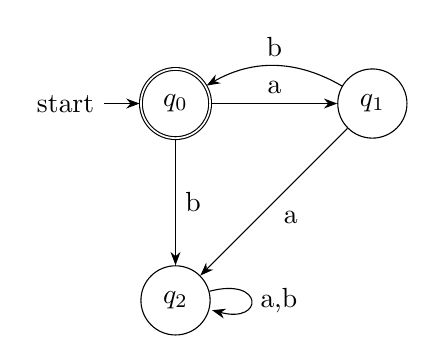
\begin{tikzpicture}[->, >=Stealth, auto, node distance=2.5cm]
			\node[initial,state,accepting] (q0) {$q_0$};
			\node[state] (q1) [right of=q0] {$q_1$};
			\node[state] (q2) [below of=q0] {$q_2$};

			\path (q0) edge node {a} (q1);
			\path (q0) edge node {b} (q2);
			\path (q1) edge [bend right] node[above] {b} (q0);
			\path (q1) edge node {a} (q2);
			\path (q2) edge [loop right] node {a,b} (q2);
		\end{tikzpicture}
		\hspace{1cm}
		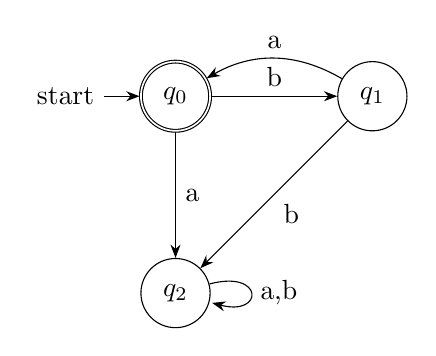
\begin{tikzpicture}[->, >=Stealth, auto, node distance=2.5cm]
			\node[initial,state,accepting] (q0) {$q_0$};
			\node[state] (q1) [right of=q0] {$q_1$};
			\node[state] (q2) [below of=q0] {$q_2$};

			\path (q0) edge node {b} (q1);
			\path (q0) edge node {a} (q2);
			\path (q1) edge [bend right] node[above] {a} (q0);
			\path (q1) edge node {b} (q2);
			\path (q2) edge [loop right] node {a,b} (q2);
		\end{tikzpicture}
	\end{center}
	\subsection{Describe the languages of $D_1$ and $D_2$}
	\begin{align*}
		L(D_1) = (ab)^*,
		L(D_2) = (ba)^*
	\end{align*}
	\subsection{Construct a DFA D such that $L(D) = L(D_1)\cap L(D_2)^c$.}
	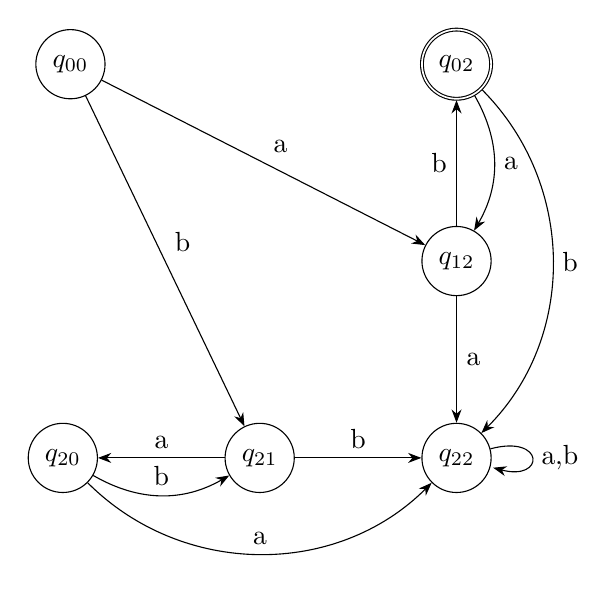
\begin{tikzpicture}[->, >=Stealth, auto, node distance=2.5cm]
		\node[state] (q00) {$q_{00}$};
		\node[state, accepting, right=4cm of q00] (q02) {$q_{02}$};
		\node[state] (q12) [below of=q02] {$q_{12}$};

		\node[state] (q22) [below of=q12] {$q_{22}$};
		\node[state] (q21) [left of=q22] {$q_{21}$};
		\node[state] (q20) [left of=q21]{$q_{20}$};


		\path (q00) edge node {a} (q12);
		\path (q00) edge node {b} (q21);

		\path (q02) edge [bend left] node {a} (q12);
		\path (q02) edge [bend left=45] node {b} (q22);

		\path (q12) edge node {a} (q22);
		\path (q12) edge node {b} (q02);

		\path (q20) edge [bend right=45] node {a} (q22);
		\path (q20) edge [bend right] node {b} (q21);

		\path (q21) edge node [above]{a} (q20);
		\path (q21) edge node {b} (q22);

		\path (q22) edge [loop right] node {a,b} (q22);
	\end{tikzpicture}

	\iffalse
	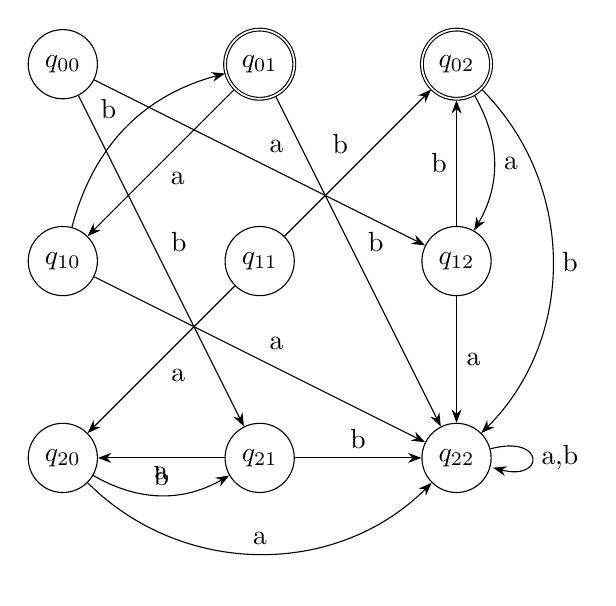
\begin{tikzpicture}[->, >=Stealth, auto, node distance=2.5cm]
		\node[state] (q00) {$q_{00}$};
		\node[state, accepting] (q01) [right of=q00] {$q_{01}$};
		\node[state, accepting] (q02) [right of=q01] {$q_{02}$};

		\node[state] (q10) [below of=q00] {$q_{10}$};
		\node[state] (q11) [right of=q10] {$q_{11}$};
		\node[state] (q12) [right of=q11] {$q_{12}$};

		\node[state] (q20) [below of=q10]{$q_{20}$};
		\node[state] (q21) [right of=q20] {$q_{21}$};
		\node[state] (q22) [right of=q21] {$q_{22}$};

		\path (q00) edge node {a} (q12);
		\path (q00) edge node {b} (q21);

		\path (q01) edge node {a} (q10);
		\path (q01) edge node {b} (q22);

		\path (q02) edge [bend left] node {a} (q12);
		\path (q02) edge [bend left=45] node {b} (q22);

		\path (q10) edge node {a} (q22);
		\path (q10) edge [bend left] node {b} (q01);

		\path (q11) edge node {a} (q20);
		\path (q11) edge node {b} (q02);

		\path (q12) edge node {a} (q22);
		\path (q12) edge node {b} (q02);

		\path (q20) edge [bend right=45] node {a} (q22);
		\path (q20) edge [bend right] node {b} (q21);

		\path (q21) edge node {a} (q20);
		\path (q21) edge node {b} (q22);

		\path (q22) edge [loop right] node {a,b} (q22);
	\end{tikzpicture}
	\fi


	\section{Exercise 4}
	Suppose we have the following language $L$ over the alphabet $\Alphabet = \set{a,b,c}$:\\
	\begin{align*}
		L = \set{w\in \Alphabet^* | w \text{ has an $a$ and every $a$ after the first $a$ in $w$ is immediately followed by a $c$}}
	\end{align*}

	\subsection{Give a regular expression $R$ such that $L(R) = L$.}
	\begin{align*}
		R = (b\cup c)^*a(b\cup c\cup ac)^*
	\end{align*}
	\subsection{Explain the answer}
	In order to enforce the one $a$ in the word, we have to go $(b\cup c)^*a(b\cup c)^*$. And then to add $ac$ blocks after the first $a$, we simply or those $ac$ blocks with the $b\cup c$.

	\section{Exercise 5}



	\section{Exercise 6}


	\section{Bonus Exercise}

\end{document}